\documentclass[10pt,a4paper]{article}
\usepackage[utf8]{inputenc}
\usepackage{amsmath}
\usepackage{amsfonts}
\usepackage{amssymb}
\usepackage{graphicx}
\usepackage{hyperref}
\author{Marco Ricci}
\title{Appunti corso Sistemi Discreti}
\begin{document}
\tableofcontents
\newpage
\section{Cyber-physical system}
Un \textbf{sistema cyber-fisico (CPS)} è l'integrazione di un processo computazionale con processi fisici il cui comportamento è definito da entrambe le parti \textit{cyber} e \textit{physical} del sistema. I computer e le reti embedded monitorano e controllano i processi fisici, di solito tramite loop di controllo (feedback loop) in cui i processi fisici influenzano le computazioni e viceversa.
\\
\subsection{Componenti di un CPS}
\begin{itemize}
\item Impianto fisico
\item Piattaforme computazionali (sensori, attuatori, computer, sistemi operativi)
\item Rete (comunicazione)
\end{itemize}

\subsection{Embedded systems}
Un \textbf{sistema embedded} è un sistema computazionale \textit{immerso} in un sistema fisico.
Ogni sistema cyber-physical contiene un sistema embedded. Nei sistemi embedded l'attenzione è focalizzata sulla parte computazionale.

Il sistema embedded non ha la rete.

\subsection{Real-time systems}
Un sistema real-time è un sistema che deve rispondere a cambiamenti esterni rispettando determinati vincoli temporali.

Molti, ma non tutti, embedded systems sono anche sistemi real-time. Ad esempio un agente automatico di trading è un sistema real-time ma non embedded. Un CPS può essere o meno un sistema real-time (auto sì, sistema audio no).

\subsection{Esempi CPS}
\begin{itemize}
\item Cardiochirurgia, ambito medico come strumenti robotici che permettono di operare anche se il chirurgo non è fisicamente presente.
\item Traffico veicolare cooperativo: auto con sistemi di assistenza alla guida. Cooperativo per scambio di messaggi tra autovetture, per sicurezza, info traffico, ridurre rischi.
\item Gestione traffico aereo: soft walls, ovvero zone proibite al volo.
\end{itemize}

\subsection{Storia del termine cyber}
L'origine del termine non proviene da \textit{cyberspace}(romanzi di William Gibson), ma dalla parola greca \textit{kybernetes}, ovvero timoniere, pilota, governatore. Venne coniato da Norbert Wiener(anni '30) come \textit{cybernetics}. Per Wiener la cibernetica è la congiunzione tra il controllo e la comunicazione.

\subsection{Sviluppo di prodotti innovativi}
Per progettare, sviluppare e implementare sistemi complessi come i CPS si adottano processi basati su un approccio che cerca di \textbf{decomporre la complessità} in piccole parti, gestire le parti e collegarle (approccio come in ingegneria del software).

\begin{itemize}
\item idea
\item modello, sul quale iniziare a fare ragionamenti
\item prototipo, sviluppato sulla base del modello, per dimostrare l'efficacia dell'idea
\item prodotto
\end{itemize}

I punti precedenti fanno parte di un processo iterativo in cui ogni fase è di un ordine di grandezza più complessa (costosa) della precedente.
Per gestire queste fasi minimizzando le probabilità di errore e ottimizzarle, ci vengono in aiuto strumenti e approcci:
\begin{itemize}
\item prototipazione virtuale, possibilità di simulare un esperimento al posto di realizzarlo fisicamente, riducendo costi e rischi se qualcosa va male. (e.g. simulazioni virtuali su auto, aerei, ecc)
\item testing delle funzionalità dei prototipi
\item verifica delle funzionalità
\item progettazione basata su modello, sistemi più o meno complicati da comprendere dove per gestire la complessità si fa riferimento a un modello.
\end{itemize}

\subsection{Processo iterativo di sviluppo}
\begin{itemize}
\item Modellazione (modeling), fase che descrive cosa fa il sistema o cosa dovrebbe fare.
\item Progettazione (design), fase che specifica come realizzare le funzionalità del sistema.
\item Analisi (analisys), fase che spiega perché un sistema fa ciò che fa ( o non fa ciò che dovrebbe fare).
\end{itemize}
\paragraph{Differenza tra sistema fisico e modello} Si utilizza la modellazione perché consente di risolvere in anticipo delle problematiche, ma il modello non è il sistema fisico, anche se esso è il più dettagliato possibile.
La scelta del modello, che sia più o meno dettagliato, dipende dal contesto in cui ci si muove. Per esempio per descrivere l'orbita degli elettroni si andrà ad utilizzare un modello tempo-discreto per questioni chimico-fisiche, perché il fenomeno ce lo richiede, ovvero la natura dell'elettrone.
Il modello utilizzato è determinato dal tipo di fenomeno/comportamento che si andrà ad analizzare, anche se l'oggetto è lo stesso.

\subsection{Buzzwords}
Una parola d'ordine è una parola o una frase, nuova o già esistente, che diventa popolare per un periodo di tempo. Le parole d'ordine spesso derivano da termini tecnici, ma spesso hanno rimosso gran parte del significato tecnico originale attraverso l'uso alla moda, semplicemente usato per impressionare gli altri.

\begin{itemize}
\item hybrid systems
\item embedded systems
\item CPS
\item Systems of systems
\item internet of things IoT\\
\end{itemize}
Per chiarire:
\paragraph{IoT} Termine utilizzato per descrivere un oggetto fisico accessibile tramite internet.
\paragraph{Embedded System} Termine utilizzato per descrivere una parte computazionale immersa nel mondo fisico
\paragraph{CPS} Termine utilizzato per descrivere una parte computazionale immersa nel mondo fisico collegate ad altre componenti tramite rete, non necessariamente internet.\\
\\
\textit{Think critically}: questi termini valgono ad oggi, ma la tecnologia cambia sempre, quindi non saranno validi o completamente validi fra qualche tempo.


CPS e controllo
La visione di IoT e CPS si estende al controllo a ciclo chiuso dei sistemi fisici.
Il controllo a ciclo chiuso non è esclusivamente una problematica ICT(controlli automatici: la comprensione della dinamica e del controllo sono fondamentali.
Un sistema stabile può diventare instabile con il controllo a ciclo chiuso e il controllo a ciclo chiuso può consentire ad un sistema instabile di comportarsi in maniera stabile.


Sfide della ricerca su CPS e controllo
Controllo su reti non deterministiche
Latenza(ritardo tra la misura e l'attuazione) e jitter(varianza del periodo di campionamento)
Larghezza di banda che influisce sullo scambio di informazioni, dati e misure
sicurezza e resilienza
sensori modelli e algoritmi plug-n-play


\section{Analisi dei dati, regressione lineare}
\marginpar{dalla video lezione 2021-09-29}
\marginpar{matlab video lezione 2021-09-29}
approccio sui dati:
la bontà del modello è legata alla bontà dei dati, ovvero se quei i dati sono rappresentativi del comportamento, dell'oggetto, del processo di nostro interesse allora il modello sarà buono. Se invece i dati sono parziali, incompleti, rappresentano pochi scenari di funzionamento del processo, è chiaro che il modello sarà limitato.

Tra i modelli che servono a descrivere processi, comportamenti quelli più semplici sono i \textbf{modelli regressivi}. Essi hanno a che vedere col legame che può esistere tra due grandezze.
Caso più semplice su slide funzione lineare. esempio persone temperatura stanza\\
caso più complesso in corrispondenza di due variabili indipendenti si ha una variabile dipendente. es valute economiche slide

l'obiettivo è sempre trovare il legame tra le variabili: ipotesi di modello

\paragraph{Ipotesi di modello\\}
Avendo a disposizione dei dati, ci si pone la domanda se i tali dati manifestano un legame, di tipo lineare o più complesso come la seconda funzione non lineare, tra le due variabili indipendenti $ u $ e $ w $ e la variabile indipendente $ y $ \\
$ y = a_{1}u+a_{2}w $\\
$ y = a_{1}u^{2}+a_{2}uw+a_{3}w^{2} $

Questi due modelli, anche essendo diversi tra loro, lineare e quadratico, possono essere gestiti con lo stesso strumento che è la regressione lineare.
La seconda equazione è risolvibile nelle incognite $  a_{1}, a_{2}, a_{3}$ perché esse compaiono in maniera lineare e \textit{u} e \textit{w} sono note, quindi valutando il legame tra le incognite e i dati e non tra le variabili dipendenti e indipendenti. Ciò vale anche se u e w o altre variabili non compaiono in modo lineare. (tabellina slide)\\
Questa peculiarità consente di applicare la stessa tecnica, basata sui minimi quadrati, per individuare i migliori valori possibili da assegnare alle incognite $ a_{1}, a_{2}, a_{3} $ per \textit{fittare} al meglio entrambi i modelli ai dati a disposizione. Questo approccio, cioè utilizzare i dati a disposizione, immaginare che il modello sia lineare nei parametri e trovare i migliori valori dei parametri, si chiama regressione lineare.

\subsection{Modelli lineari}
Problema: \textbf{stimare la retta ai minimi quadrati} che meglio approssima il legame tra una variabile indipendente \textit{x} una dipendente \textit{y}.\\
Il modello cercato è del tipo $ y=ax+b $\\
e deve \textit{fittare} tutti i dati a disposizione.

Per individuare il modello in maniera univoca, di quanti parametri si ha bisogno?
Due: coefficiente angolare \textit{a} e l'intercetta \textit{b}. Riformulo il problema: trovare i valori di \textit{a} e \textit{b} che consentono di fittare il modello a tutti i dati a disposizione. Per dati a disposizione si intendono tutti i valori di x e y, rappresentati magari in tabelle(tipo funzione).
Per individuare a e b bastano due equazioni (due righe di tabella), dato che il sistema è di tipo lineare a due incognite. 
Se a disposizioni ci sono 10 righe, quali tra queste andrebbero prese?

scostamento, sistema di equazioni approssimate, 

Si assume che l'equazione approssimata possa diventare esatta aggiungendo il termine $e_{i}$, errore di equazione, scostamento.\\

$ y_{i}=ax_{i}+b+e_{i} $\\
Si aggiunge \textit{e} altrimenti il sistema sarebbe approssimato: $ y_{i} \sim ax_{i}+b $

Con l'aggiunta di \textit{e} bisogna risolvere il sistema anche rispetto ad essa. Non rappresenta una terza incognita, perché il numero di \textit{e} è pari al numero di equazioni.
Ora il numero di incognite sarà il numero di e + i due parametri a e b. Il sistema non è risolvibile poiché si hanno più incognite che equazioni.\\

riepilogo sistemi di equazioni \marginpar{videolezione 2021-10-04 min ~30}\\

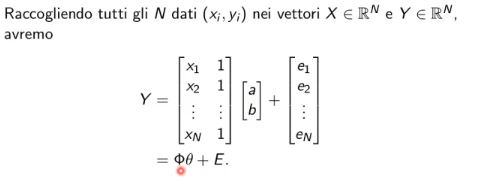
\includegraphics[scale=0.61]{matri.png} 
incognite: a, b, E.

Questo procedimento, valido per la retta ai minimi quadrati, si può estendere a qualsiasi tipo di modello di regressione lineare. L'importante è che si è in grado di scrivere il valore della variabile dipendente $ y_{i} $ in forma vettoriale, dove si ha il vettore delle incognite teta, il vettore riga dei regressori fi con i, \\
$ y_{i}=\varphi_{i}^{T} \theta+e_{i} $\\
questo modo di scrivere i dati è quello più generale possibile per un modello di regressione lineare, poiché le incognite sono in $ \theta $ che compare in forma lineare

con un numero di incognite maggiore del numero di equazioni si ottengono infinite soluzioni. Tra queste infinite soluzioni, praticamente, quale va scelta?
Qui interviene l'approccio dell'ottimizzazione, ovvero la scelta della soluzione ottima, migliore rispetto ad un determinato criterio. Esempio di criterio la retta ai minimi quadrati, che prende la retta che rende il più piccolo possibile l'errore quadratico medio. In questo caso gli errori sono contenuti nel vettore E

Errore quadratico medio $ \dfrac{1}{N} \sum_{i=1}^N e_{i}^{2} $

Bisogna prendere valori di $ \theta $ tali che l'errore quadratico medio sia piccolo.
Come si ottengono i valori di $e_{i}$?
$y_{i}$ e $ \varphi_{i}^{T} $ sono note quindi: $ e_{i}=y_{i}-\varphi_{i}^{T} \theta $
$ e_{i}(\theta) $ dipende da $ \theta $

Tutte le componenti dell'errore saranno in funzione di $ \theta $.

il problema di regressione lineare consiste nel risolvere questo problema di ottimizzazione:\\
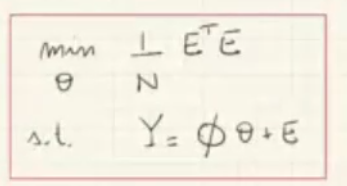
\includegraphics[scale=0.41]{err.png} \\
in cui 





\section{Modelli Dinamici}
Finora abbiamo visto come queste tecniche di regressione lineare possono essere applicate per modellare e stimare dei legami di tipo statico. statico ossia funzioni tra regressori e misure.
Le stesse tecniche possono essere applicate anche per modellare dei comportamenti di tipo dinamico.
\subsection{Identificazione modelli dinamici}
L'applicazione di tecniche di regressione lineare al caso di modelli dinamici porta a quella disciplina dei controlli che si chiama \textbf{identificazione dei modelli dinamici}. Dinamico i dati che andiamo a misurare dipendono dal tempo, quindi dalla storia precedente e dall'evoluzione del modello stesso. 
Per modellare questo comportamento andiamo ad utilizzare un modello dinamico descritto dall'equazione alle differenze di ordine \textit{p}.
Finora avevamo detto che le misure dipendevano da alcune variabili indipendenti. In questo caso andiamo a modellare il comportamento dinamico di una variabile.

\begin{equation}
y(k)=a_{1}y(k-1)+a_{2}y(k-2)+...+a_{p}y(k-p)
\end{equation}

L'idea è quella di immaginare che il fenomeno possa essere espresso come combinazione lineare dei valori che la variabile y, mia misura, aveva ai passi precedenti.

Ci sono analogie con le tecniche utilizzate in precedenza: $ y(k) \longleftrightarrow y_{i} $  \\ \\
e i valori della variabile al passo precedente saranno l'equivalente dei valori dei regressori del modello di regressione lineare $ [y(k-1) \, y(k-2)...y(k-p)]\longleftrightarrow \varphi_{i}^{T} $ \\ \\
così come i coefficienti dell'equazione alle differenze sono i parametri della regressione lineare da identificare:
$ [a_{1}\,a_{2}\,...\,a_{p}]_{T} \longleftrightarrow \theta $ \\
A questo punto, portatici nel caso della regressione lineare ($ y_{i}=\varphi_{i}\theta $), possiamo applicare la tecnica di ottimizzazione ai minimi quadrati e trovare i valori di $ [a_{1}\,a_{2}\,...\,a_{p} $ che meglio approssimano in termini di errore quadratico medio l'equazione ricorsiva(eq. 1).
Questo modello dato dall'eq 1 è detto modello \textbf{autoregressivo}, poiché è una regressione fatta su se stesso.
Ma se ho un modello AR, le osservazione da cosa dipendono? Dalle osservazioni precedenti, si dice quindi che il sistema è autonomo, non ha bisogno di interagire col mondo esterno e non c'è modo di influenzare le osservazioni.(e.g. andamento titolo azionario)\\

Qualora volessimo avere una relazione con altri dati, l'equazione alle differenze può essere modificata aggiungendo una combinazione lineare di un ingresso esogeno, esterno:\\
\begin{equation}
y(k)=a_{1}y(k-1)+...+a_{n}y(k-n)+b_{0}u(k)+b_{1}u(k-1)+\,...\,+b_{m}u(k-m)+e(k)
\end{equation}
questo è detto modello autoregressivo esogeno (ARX).
L'equazione alle differenze è di ordine \textit{n} (occorre tener memoria degli \textit{n} valori precedenti della \textit{y per generare il valore corrente}) ed il numero dei parametri del modello è pari a p=n+m+1.

\subsection{Algoritmo LMS: Least Mean Square}
\marginpar{videolezione 2021-10-11}
Algoritmo per risolvere problemi di regressione lineare.
Come sempre, il modello che andiamo ad individuare dipende dai dati a nostra disposizione. La bontà del modello, parametri vicini ai valori veri, dipende da quanto i dati a disposizione siano rappresentativi del comportamento del sistema, fenomeno.
Se le osservazioni fatte sono legate soltanto a un piccolo aspetto, una specifica fase del processo, ma non tutto il range del comportamento del processo stesso. Quindi $ \theta $ è funzione di $\phi$ e $y$, e $\phi$ e $y$ hanno a che fare con le osservazioni e con i dati del sistema.\\
\textit{(Garbage in, Garbage out)}\\
Ci si potrebbe basare anche sul fatto che più osservazioni vengono fatte, più è probabile che il modello stia ricoprendo ogni aspetto del sistema e che non sia legato a soli certi aspetti specifici. Quindi se le osservazioni sono molte, equidistribuite, non polarizzate, ci avvicineremo di più ai valori "veri".

Ma quando possiamo fare la prima stima? quante osservazioni prima della stima dei parametri?
Se ho 50 osservazioni, aspetto che ne arrivino altre? e quando arrivano faccio la stima delle nuove o metto tutto insieme e stimo?\\

Ogni volta volta che arriva una nuova osservazione l'equazione normale(matrice di eq norm) va riformulata e risolta, non elaborando solo la nuova misura.
Questo algoritmo è detto minimi quadrati a lotti, lotti perché per risolvere devo vere tutte le osservazioni memorizzate.

Meglio sarebbe avere un algoritmo che dopo una nuova misura il nuovo vettore dei parametri deve essere aggiornato, e per aggiornarlo devo osservare solo la nuova osservazione e capire di quanto scostarmi dal vecchio valore dei parametri.\\

Algoritmo che esprime la nuova misura in funzione del valore del parametro precedente si chiama \textbf{RLS}, minimi quadrati ricorsivi.
Molto comodo perché può funzionare sempre, ad ogni osservazione, anche in realtime.

\textbf{Least mean square, minimo errore quadratico medio}
Abbiamo ipotizzato il modello di regressione lineare:
\begin{equation}
h_\theta(x)=\varphi^T\theta=\theta_0+\sum_{j=1}^{p-1}x_j\theta_j
\end{equation}
dove $ \varphi $ è il vettore riga dei regressori e $ \theta $ è il vettore dei parametri.
Con il modo di scriverlo in sommatoria, viene evidenziato il termine noto $ \theta_0 $, mentre gli altri parametri vanno a moltiplicare gli altri valori delle variabili indipendenti.
La funzione da minimizzare è l'errore quadratico medio:
\begin{equation}
J(\theta)=\frac{1}{2} \sum_{i=1}^N(y^{(i)}-h_{\theta}(x^{(i)}))^2
\end{equation}
cioè l'osservazione meno la stima ottenuta utilizzando i parametri e il vettore dei regressori.

Come si risolve il problema ai minimi quadrati formulato in questa maniera?
Col gradiente:\\
$ \dfrac{\partial}{\partial \theta_j}J(\theta)=-\sum_{i=1}^N((y^{(i)}-h_\theta (x^{(i)}))x_j^{(i)} $
qui si ragiona in termini di scalari, quindi con la componente j-esima del gradiente
L'algoritmo che si può implementare è l'algoritmo, non ai minimi quadrati a lotti che ci dà in un colpo solo la soluzione del problema di ottimizzazione, ma uno basato sulla discesa del gradiente. Simile alla ricerca del minimo di una funzione(derivata = 0) fatto in maniera iterativa, applicato al caso a più variabili.
In maniera analitica il minimo si calcola in un colpo solo, direttamente risolvendo un'equazione, imponendo la derivata=0.
Se volessimo farlo fare a un calcolatore l'idea è quella di muoversi per tentativi, in maniera iterativa, muovendosi nella direzione della derivata che fa decrescere la funzione. Inizia da un valore a caso, valuta il valore della funzione e valuta il valore della derivata che la funzione assume in quel punto. Poi da quel punto si muove nella direzione opposta al valore della derivata perché la derivata dice la tangente a quel punto, se la derivata è positiva vuol dire che muovendosi nella direzione della derivata la funzione cresce. Dato che cerchiamo il minimo, ci si muove nella direzione opposta al valore della derivata e continuo a fare l'update dei tentativi finché lo scostamento ottenuto è piccolo. Piccolo significa che la derivata è piccola perché si trova nell'intorno di un punto di minimo. Questa è la tecnica della discesa del gradiente, cerca il punto di minimo nel caso multivariabile (caso scalare uso la derivata) e consiste nel cercare in maniera iterativa il punto di minimo andando a valutare sempre nuovi valori che si muovono in direzione opposta al gradiente. Opposta perché vado nella direzione in cui la derivata diventa sempre più negativa, decresce la funzione.
Nel caso multivariabile guardo il gradiente e ciò che va aggiornato è $ \theta $ ad ogni iterazione. Il nuovo $ \theta $ sarà dato dal $ \theta $ corrente più lo scostamento.

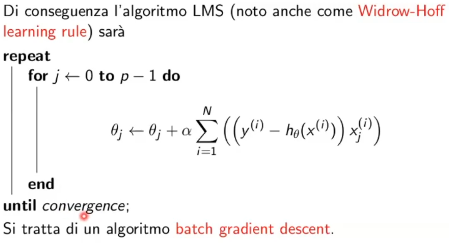
\includegraphics[scale=0.41]{lms.png} 

differenze rispetto ai minimi quadrati a lotti:
non lavora con matrici, solo funzioni scalari
lavora maniera iterativa
non conosco il tempo di risoluzione del problema a priori
in ogni caso si converge
scelta adeguata del parametro alfa\\ \\ \\

Quando i dati a disposizione sono tanti $ N\rightarrow\infty $ si può decidere di aggiornare tutti i parametri usando un dato per volta:\\

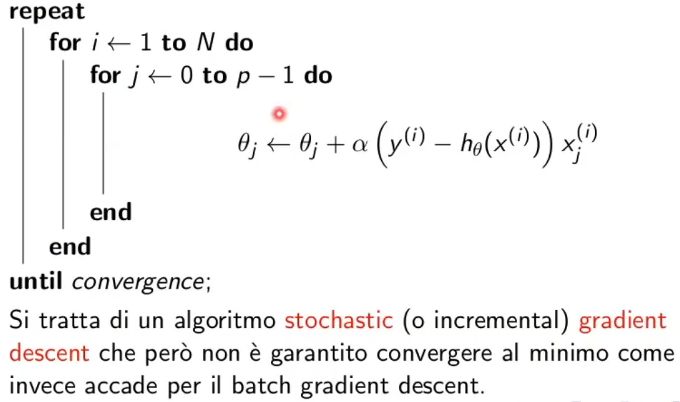
\includegraphics[scale=0.41]{lms2.png} 



































\end{document}